\begin{recipe}
    [% 
        preparationtime = {\unit[0.5]{h}},
        portion = {\portion{3-4}},
        bakingtime = {\unit[0.5]{h}}
    ]
    {Tart with beetroot and goat cheese}
    
    \introduction{%
        This tart is sooo easy to do.
        And quite spectacular.
        Add salad, wine, candles... more wine ;)
    }

    \ingredients{%
        & Puff pastry \\
        3 & Cooked/baked beetroot \\
        \unit[200]{g} & Goat cheese \\
        4 & Eggs \\
        \unit[200]{ml} & Sour cream \\
        1 tbs. & Flour \\
        & Thyme \\
        & Balsamic vinegar
    }

    \preparation{%
        \step Mix eggs, cream, flour and spices.

        \step Slice beetroot and goat cheese.

        \step Line oven dish with puff pastry, make a few holes with a fork.
        Blind bake for 5 min.

        \step Layer beetroot, then cheese.
        Pour over egg mixture. \underline{Bake for 25-30 min at \unit[180]{\textcelcius}.}

        \step  Sprinkle with balsamic vinegar.
    }

\end{recipe}

\begin{figure}[h]
    \centering
    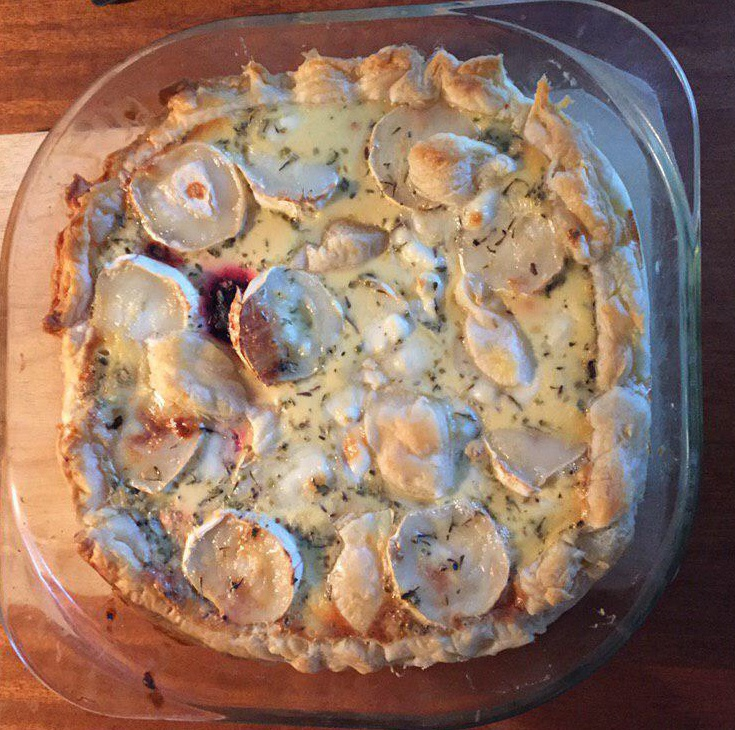
\includegraphics[height=9cm]{pic/beetroot_cheese}
\end{figure}
